\section{Modelo final}\label{sec:final}

\subsection{Arquitectura}
El modelo recibe tres entradas por parcela, el régimen codificado en dos columnas indicadoras (A o B) y el rezago
espacial estandarizado. Un proceso gaussiano~\cite{rasmussen2006} predice el rendimiento suponiendo que parcelas con
entradas parecidas tienen rendimientos parecidos. Qué tan parecidas lo define la covarianza
\begin{equation}
k(\mathbf{x},\mathbf{x}') = \sigma_f^2 \exp\!\left(-\frac{\lVert\mathbf{x}-\mathbf{x}'\rVert^2}{2\lambda^2}\right) +
\sigma_n^2\,\delta_{\mathbf{x}\mathbf{x}'} ,
\label{eq:kernel}
\end{equation}
donde $\lambda$ es la distancia a la que dos parcelas dejan de parecerse, $\sigma_f^2$ la variación que explica el
modelo y $\sigma_n^2$ el ruido que no explica. Los tres se ajustan maximizando la verosimilitud. Dentro de
la validación se reajustan en cada fold usando solo las parcelas de entrenamiento de ese fold. En los 50 folds de
validación varían entre 0.51 y 1.41 para $\sigma_f^2$, entre 0.87 y 2.62 para $\lambda$ y entre 0.21 y 0.35 para
$\sigma_n^2$, sin tocar las cotas permitidas. El modelo final, que se entrega para predecir las 59 parcelas, se ajusta
con las 138 parcelas y queda con $\sigma_f^2=0.77$, $\lambda=1.57$ y $\sigma_n^2=0.26$, en unidades del rendimiento
estandarizado. Es decir, el modelo atribuye cerca de una cuarta parte de la variación a ruido. Lo que sí elegimos
viendo las 138 parcelas es la estructura del modelo, como el radio de 400\,m, los 10 vecinos y el algoritmo. El costo de
esa elección lo mide la validación anidada de la Sección~\ref{sec:confiabilidad}.

\subsection{Error de predicción}
En el esquema A el modelo obtiene un RMSE de 0.458\,t/ha, un error absoluto medio de 0.312 y un $R^2$ de 0.71. Mejora a
la media por régimen en los dos regímenes, de 0.535 a 0.494 en el A y de 0.398 a 0.389 en el B. En el esquema B empata
con ella (0.489), como se espera, porque sin vecinos cercanos el rezago se convierte en la media del régimen.

La Fig.~\ref{fig:obspred} muestra la limitación principal. Las predicciones forman dos franjas, una por régimen, y
dentro de cada una varían poco. Su desviación es cerca de 0.4 veces la de las etiquetas. El modelo acierta el nivel del
régimen y corrige con los vecinos, pero las parcelas con rendimientos extremos, como las de 5.5\,t/ha en
Chignahuapan, quedan cerca de la media. No forzamos más dispersión, porque sin información que la respalde subiría el
error.

\begin{figure}[t]
\centering
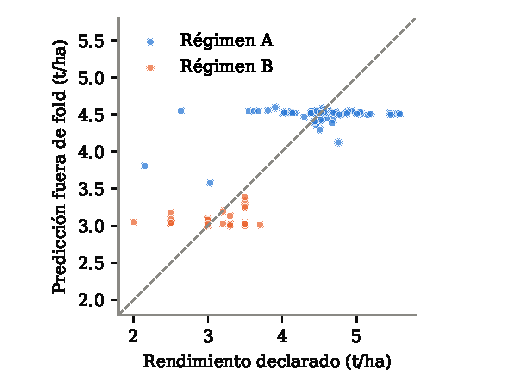
\includegraphics[width=0.9\columnwidth]{f6_observado_predicho}
\caption{Rendimiento declarado contra predicción fuera de fold, promedio de las 10 repeticiones. La línea punteada es
la predicción perfecta.}
\label{fig:obspred}
\end{figure}

\subsection{Intervalos de predicción}
Para FIRA, que evalúa crédito, importa también cuánto puede fallar cada predicción. Cada parcela recibe un intervalo
del percentil 10 al 90 calculado con predicción conformal dividida~\cite{vovk2005,lei2018}, en su variante de Mondrian,
que calibra por separado en cada grupo, aquí cada régimen~\cite{vovk2005}. El método tiene tres pasos. Primero,
guardamos los errores con signo $r=y-\hat y$ de las predicciones fuera de fold, es decir, de parcelas que el modelo no
vio, en las 10 repeticiones de la validación cruzada. Son 1380 errores, 870 del régimen A y 510 del B. Segundo, para cada
régimen calculamos los cuantiles 0.10 y 0.90 de sus errores. En el A valen $-0.51$ y $+0.57$, y en el B $-0.55$ y
$+0.48$\,t/ha. Tercero, el intervalo de una parcela es p10 igual a la predicción más el cuantil 0.10 de su régimen, y
p90 igual a la predicción más el cuantil 0.90. Como los cuantiles tienen signo, el intervalo no es simétrico. Los 1380
errores son 138 parcelas repetidas 10 veces, así que la calibración equivale a 87 parcelas en el A y 51 en el B. Con los
mismos errores estimamos la probabilidad de que el rendimiento quede por debajo de 2.5\,t/ha.

Para medir si el intervalo cumple, usamos validación anidada, en la que la parcela evaluada no participa ni en el
ajuste ni en la calibración (Fig.~\ref{fig:cobertura}). La cobertura total es 0.826, que son 570 aciertos en 690
evaluaciones (138 parcelas por 5 repeticiones), con un ancho medio de 1.13\,t/ha. Como cada parcela se evalúa cinco
veces, calculamos el intervalo de confianza del 95\,\% con un bootstrap por parcela y resulta de 0.765 a 0.883, que
incluye la meta de 0.80. Por régimen la cobertura es 0.791 en el A (intervalo de 0.708 a 0.869) y 0.886 en el B
(de 0.816 a 0.949). En el cuartil de parcelas más chicas es 0.77 (de 0.63 a 0.90). Con 35 parcelas por cuartil, esta
diferencia no es concluyente y la tratamos solo como una observación exploratoria.

\begin{figure}[t]
\centering
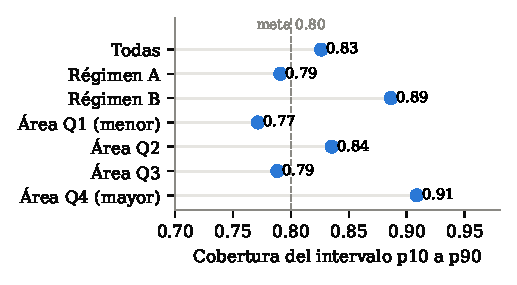
\includegraphics[width=\columnwidth]{f10_cobertura}
\caption{Fracción de parcelas cuyo rendimiento cae dentro de su intervalo p10 a p90, por régimen y por cuartil de
área. La meta es 0.80.}
\label{fig:cobertura}
\end{figure}

\subsection{Predicciones de las 59 parcelas}
El Cuadro~\ref{tab:predicciones} del apéndice lista las 59 predicciones con sus intervalos. Las 37 parcelas del régimen A tienen una predicción media de 4.49\,t/ha (de 3.72 a 4.58) y las 22 del B de 3.06\,t/ha
(de 2.75 a 3.66), igual que las medias de entrenamiento (Fig.~\ref{fig:mapa}). Ninguna sale del rango observado en
su régimen. La probabilidad de quedar bajo 2.5\,t/ha supera 0.10 en 18 parcelas, todas del régimen B.

\begin{figure}[t]
\centering
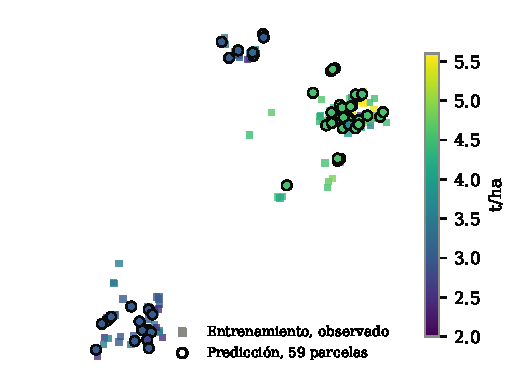
\includegraphics[width=0.95\columnwidth]{f12_mapa}
\caption{Rendimiento observado en las parcelas de entrenamiento (cuadros) y predicho en las 59 parcelas (círculos con
borde), con la misma escala de color. Los grupos en tonos oscuros, al oeste, son del régimen B.}
\label{fig:mapa}
\end{figure}
